\documentclass[aspectratio=43]{beamer}
\usetheme{Berlin}

\usepackage[czech]{babel}
\usecolortheme{dolphin}
\usepackage{graphicx}
\usepackage{dirtree}
\usepackage{listings}
\usepackage[T1]{fontenc}
\usepackage{lmodern}
\usepackage[utf8]{inputenc}
\usepackage{caption}
\usepackage{bbding}
\usepackage{xurl}
\usepackage{scrextend}
\usepackage{minted}
\usepackage{appendixnumberbeamer}

\captionsetup{labelformat=empty}

\beamertemplatenavigationsymbolsempty
\defbeamertemplate*{title page}{customized}[1][]
{
	\usebeamerfont{title}\inserttitle\par
	\usebeamerfont{subtitle}\usebeamercolor[fg]{subtitle}\insertsubtitle\par
	\bigskip
	\usebeamerfont{author}\insertauthor\par
	\usebeamerfont{institute}\insertinstitute\par
	\usebeamerfont{date}\insertdate\par
	\usebeamercolor[fg]{titlegraphic}\inserttitlegraphic
}

\hypersetup{unicode}
\hypersetup{breaklinks=true}


\title{Bezpilotní letadlo}
\subtitle{dron postavený na platformě Raspberry Pi}
\author{Havránek Kryštof 4.E}
\date{7. března 2022}
\institute{Gymnázium, Praha 6, Arabská 14}
\setbeamertemplate{sidebar right}{}
\setbeamertemplate{footline}{%
\hfill\textbf{Stránka \insertframenumber{}. z \inserttotalframenumber} \hspace{0.01cm} \vspace{0.1cm}}
\setbeamerfont{footnote}{size=\tiny}

\begin{document}

\begin{frame}[plain]
	\maketitle
\end{frame}

\clearpage
\setcounter{framenumber}{0}

\begin{frame}[fragile]
	\frametitle{Úvod}
	\section{Úvod}

	\begin{itemize}
		\item Bezpilotní letadlo a jeho dobrovolný systém -- dálkové řízené, přenos videa a telemetrie
		\item Proč jsem si téma vybral? % zajímá mně hardware a po konfliktu na náhorním karabachu mě zaujalo téma dronů. S modelářstvím jsem navíc neměl žádné předchozí zkušenosti a práce tak byla dobrým začátečním bodem
		\item Kód dostupný na GitHubu pod licencí MIT (včetně knihoven)
		\item Linux + Raspbian, port ovládacího software je možný
		\item řízení přes Xbox ovladač
	\end{itemize}
\end{frame}

\begin{frame}[fragile]
	\frametitle{Protokol}
	\begin{itemize}
		\item komunikace prostřednictvím TCP protokolu
		\item video předáváno přes UDP
		\item protokol navržený pro potřeby práce -- tři základní funkce -- telemetrie, ovládání a nastavení
		\item předávání struktur
		\item Raspberry Pi -- server, Pilot -- klient
		\item podpora více ovládacích stanic
	\end{itemize}
\end{frame}

\begin{frame}[fragile]
	\frametitle{Design letadla}
	\section{Design letadla}
	\begin{itemize}
		\item založeno na kostře Mini Talon od společnosti X-UAV
			\begin{itemize}
				\item rozpětí křídel: 130cm
				\item délka: 85cm
				\item vzletová váha: 1.5 kg
			\end{itemize}
		\item délka letu nad 1 hodinu
		\item jádro -- Raspberry Pi Zero 2
		\item doprovázen řadou periférií
	\end{itemize}
\end{frame}

\begin{frame}[fragile]
	\frametitle{Design letadla}
	\begin{figure}[h]
		\centering
		\includegraphics[height=7cm]{./../img/photo1.jpg}
	\end{figure}
\end{frame}

\begin{frame}[fragile]
	\frametitle{Design letadla}
	\begin{figure}[h]
		\centering
		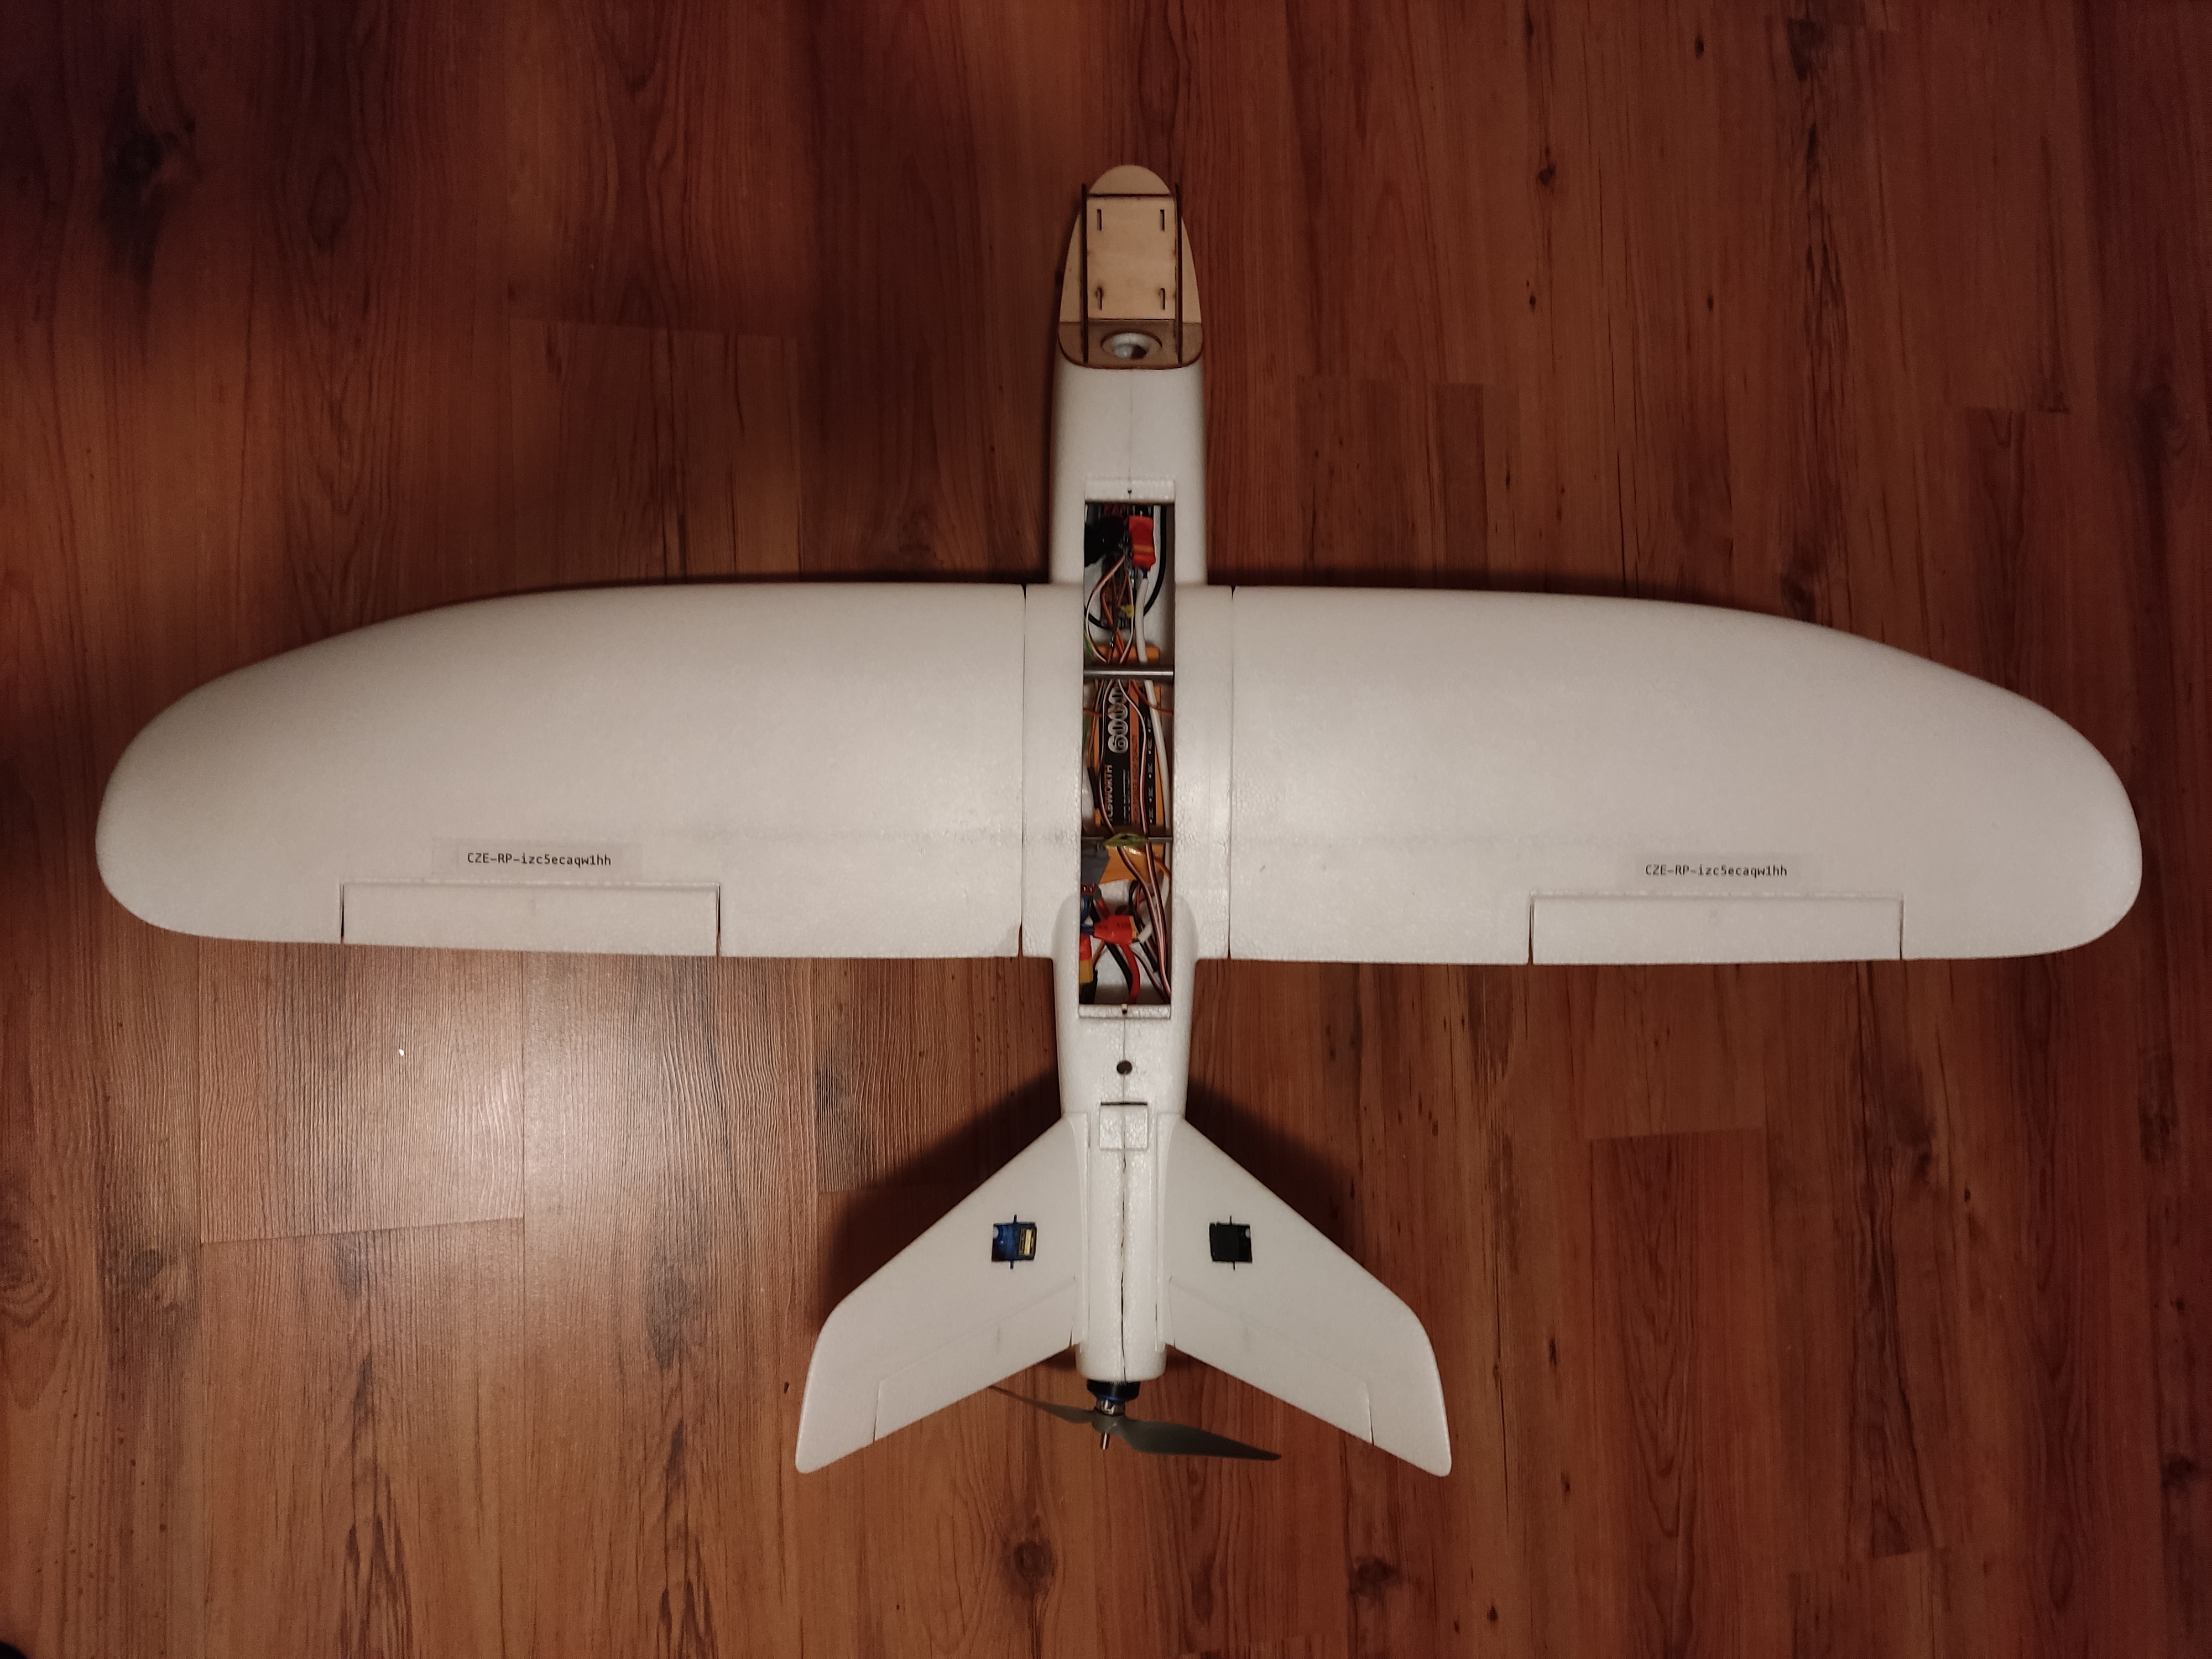
\includegraphics[height=7cm]{./../img/whole_plane.jpg}
	\end{figure}
\end{frame}


\begin{frame}[fragile]
	\frametitle{Periférie}
	\begin{itemize}
		\item Wit-Motion WT901B
			\begin{itemize}
				\item devíti osý polohový senzor
				\item údaje o orientaci v prostoru, teplotě, zrychlení
				\item slouží k fungování autopilota
			\end{itemize}
		\item INA226
			\begin{itemize}
				\item voltmetr/ampér metr
				\item měří odběr celého letadla a napětí na baterii
			\end{itemize}
	\end{itemize}
\end{frame}

\begin{frame}[fragile]
	\frametitle{Periférie}
	\begin{itemize}
		\item ublox NEO 7M
			\begin{itemize}
				\item GPS modul
				\item údaje o poloze a nadmořské výšce
			\end{itemize}
		\item PCA9865
			\begin{itemize}
				\item modul na ovládání servo motorů
				\item připojen na ESC (Beatles 40A) -- ovládá rychlost hlavního motoru
			\end{itemize}
	\end{itemize}
\end{frame}

\begin{frame}[fragile]
	\frametitle{Zapojení}
	\begin{figure}[h]
		\centering
		\includegraphics[height=7cm]{./../img/schema.png}
	\end{figure}
\end{frame}

\begin{frame}[fragile]
	\frametitle{Zapojení}
	\begin{figure}[h]
		\centering
		\includegraphics[height=7cm]{./../img/circuit.jpg}
	\end{figure}
\end{frame}

\begin{frame}[fragile]
	\frametitle{Program letadla}
	\begin{itemize}
		\item se senzory se komunikuje prostřednictvím knihoven
			\begin{itemize}
				\item 3 fouknuté a přepsané knihovny
				\item v programu se přistupuje přes singletony, které činní operace thread safe
			\end{itemize}
		\item stream z kamery je aktuálně spuštěn programem v podprocesu
		\item za standardního provozu se letadlo řídí pokyny pilota
		\item čekání na zprávu $\Rightarrow$ vyhodnocení $\Rightarrow$ thread pool zpracuje
		\item letadlo je schopno držet svojí letovou hladinu -- dva PID kontroléry
	\end{itemize}
\end{frame}

\begin{frame}[fragile]
	\frametitle{Ovládací software}
	\section{Ovládací software}
	\begin{itemize}
		\item vyvíjen pro operační systém Linux
		\item postavený na grafickém toolkitu Gtk3
		\item zpracování dat z ovladače, zobrazení videa a telemetrie
		\item ovladač
			\begin{itemize}
				\item použit návrhový vzor observeru -- interface s ovladačem generuje události
				\item nemusí tak existovat centrální organizační bod
			\end{itemize}
	\end{itemize}
\end{frame}

\begin{frame}[fragile]
	\frametitle{Ovládací software}
	\begin{figure}[h]
		\centering
		\includegraphics[height=7cm]{./../img/interface.png}
	\end{figure}
\end{frame}


\begin{frame}[fragile]
	\frametitle{Závěr}
	\section{Závěr}
	\begin{itemize}
		\item cíl práce byl splněn
		\item práce však nebyla realizována v původně zamýšleném rozsahu
		\item řada problémů, kritický nedostatek znalostí
		\item kvádrokoptéra x dron x letadlo
	\end{itemize}
\end{frame}

\begin{frame}[fragile]
	\frametitle{Budoucnost Projektu}
	\begin{itemize}
		\item upozornění na letovou zónu
		\item spojení s ATAK
		\item autopilot
		\item přechod od Wi-Fi, rezervní spojení?
		\item doprovodný hardware -- tracking anténa, katapult
	\end{itemize}
\end{frame}


\end{document}
